\documentclass{entcs}
\usepackage{entcsmacro}
%NOTE: oz.sty clashes with entcs.cls, so we use a hacked version of oz.sty
\usepackage{czt}
\usepackage{graphicx}

% Extra general macros for this paper.
\newenvironment{Rationale}{\\ \textbf{Rationale:}\it}{}

% Extra math-mode macros for this paper.
% Some of these may eventually go into czt.sty
\newcommand{\V}{\mathcal{V}}
\newcommand{\Zc}{Z_C}

\def\lastname{Utting, Malik, Toyn}

\begin{document}
\begin{frontmatter}
  \title{Transforming Z with Rules}
  \author{Mark Utting\thanksref{emailMark}}
  \address{Department of Computer Science\\
    The University of Waikato\\
    Hamilton, New Zealand} 
  \author{Petra Malik\thanksref{emailPetra}}
  \address{Department of Computer Science\\
    The University of Waikato\\
    Hamilton, New Zealand} 
  \author{Ian Toyn\thanksref{emailIan}}
  \address{Department of Computer Science\\
    The University of York\\
    Heslington, York, UK}
  \thanks[emailMark]{Email: \texttt{marku@cs.waikato.ac.nz}}
  \thanks[emailPetra]{Email: \texttt{petra@cs.waikato.ac.nz}}
  \thanks[emailIan]{Email: \texttt{ian@cs.york.ac.nz}}
\begin{abstract}
  This paper describes a simple extension of Z that allows transformation
  and reasoning rules to be written in a natural, Z-like notation.  This
  gives a high-level, declarative way of specifying transformations of Z
  terms, which makes it easier to build new Z manipulation tools.
  We describe the syntax and semantics of these rules, plus several reasoning
  engines that use sets of rules to manipulate Z terms.  We demonstrate the
  utility of rules by discussing one set of rules that defines schema
  unfolding of the schema expressions in Z and another set that is used by
  the ZLive animator to preprocess Z expressions into a form more suitable
  for animation.  
\end{abstract}
\begin{keyword}
  Z, CZT, reasoning, rewriting rules
\end{keyword}
\end{frontmatter}



\section{Introduction}

In many Z tools, schema unfolding and other Z transformations are performed
by large amounts of low-level code (for example, in C or Java) that
manipulate the syntax of Z schema expressions and return equivalent
unfolded terms.  This low-level approach is error-prone, and the code that
performs the transformations is time-consuming to write and difficult to
read.  The problem is that the essence of the abstract transformations are
hidden in the masses of low-level code.

This means that building new Z transformation tools is time-consuming,
requires programming skills, and also requires detailed knowledge of the
API for manipulating Z syntax trees.  In contrast, in an ideal world, it
should be quick and easy to define new Z transformations by writing them in
the Z notation itself, in a high-level, declarative style that is easily
understood and can perhaps even be proven correct according to some given Z
logic.  A high-level notation such as this gives better support for the
capture and reuse of the knowledge implicit in the rules~\cite{DenningACM}.

This paper proposes such a declarative notation, called ZedRules.
It is an extension of the standard Z notation that provides \emph{jokers}
that can stand for arbitrary expressions, predicates, declarations etc.
It allows equality and inference rules to be written in a Z-like notation,
and users can extend this notation by defining new operators within Z.

Section \ref{sec:syntax} describes the syntax and semantics of the
ZedRules.  Section~\ref{sec:engines} describes three different reasoning
engines provided by CZT to use the rules.  Section~\ref{sec:schemas} shows
how the rules can be used to specify unfolding and normalisation of schema
expressions and Section~\ref{sec:zlive} shows some of the rules that are
used by ZLive to preprocess Z expressions and predicates.



\section{Related Work}


\section{Rule Syntax and Semantics}

This section describes the syntax and semantics of the Z rules.

Each rule has a single conclusion and possibly several antecedents, so is a
horn clause.  Thus we have a high-level Prolog-like notation (but with Z
syntax) for defining Z transformations and automatic proofs.

We describe the semantics of the rules independently of any operational
description of how rules can be used. 

This allows rules to be used by many different reasoning and rewrite
engines.  Each engine may place different restrictions on the rules
that it allows, may apply rules using a different semantics (apply once,
apply exhaustively, apply to all subterms bottom-up or top-down etc.), and
may use a different implementation technology (for example, an interpreter
that applies the rules or a compiler that transforms the rules into Java
code).


\section{Tools for Rules}


\subsection{A Simple Interactive Prover}

\begin{figure}[htbp]
  \centering
  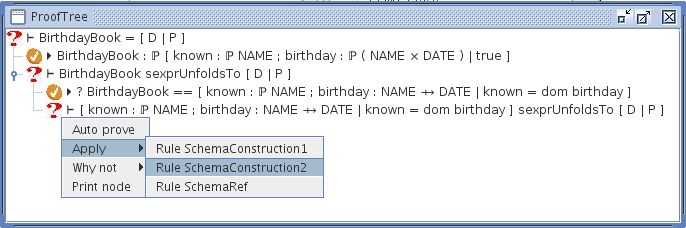
\includegraphics[width=\textwidth]{cztprover1}
  \caption{Screenshot of Interactive Prover}
  \label{fig:cztprover}
\end{figure}


\subsection{An Automated Depth-First Prover}

\subsection{A Rewrite Engine}

\section{Example Rules: Schema Unfolding}

\section{Example Rules: ZLive Preprocessor}

\section{Conclusions}


TODO: conclusions


In the future, we would like to be able to extend the ZedRules notation to
support a variety of Z logics, such as
$Z_C$~\cite{henson:revising-z-1-99,henson:revising-z-2-99},
$\mathcal{V}$~\cite{brien:calculus-schemas-z00} (a successor of the
$\mathcal{W}$ logic that appeared in early drafts of the Z standard).  It
is desirable to support both $Z_C$ and $\mathcal{V}$ (and any future
proposals for Z logics), since they are rather different and it would be
interesting to compare them in a common framework.  For example,
substitution is a meta-level operation in $Z_C$, but is defined within the
object logic of $\mathcal{V}$.

The current CZT reasoning tools construct an explicit proof tree that
allows proofs to be recorded, replayed, displayed, checked by independent
tools etc.
It would be interesting to build a tactic layer on top of this proof
tree, using a tactic language such as ANGEL~\cite{martin:tactics}, which
has been used as the basis of several other Z provers (CadiZ, Jigsaw1,
Jigsaw2, Ergo).  This would make it easier to program combinations of rules
in flexible ways, whereas currently such tactics must be written in Java.

In the future, we would also like to be able to translate the rules
into a form that Z theorem provers can accept, so that we can prove
rules correct --- a simple declarative semantics for rules makes this
easier to achieve.

\end{document}
